\documentclass{beamer}
%\documentclass[handout]{beamer}

% language settings
%\usepackage{fontspec, polyglossia}
%\setdefaultlanguage{magyar}

% common packages
\usepackage{amsmath, multimedia, hyperref, color, multirow}
%\usepackage{graphicx}

% TikZ
\usepackage{tikz}
%\usetikzlibrary{arrows.meta, decorations.pathmorphing, decorations.pathreplacing, shapes.geometric,mindmap}
%\usetikzlibrary{shapes.geometric,fadings,bayesnet}

% beamer styles
\mode<presentation>{
\usetheme{Madrid}
%\usetheme{Antibes}
\usecolortheme{beaver}
%\usecolortheme{seahorse}
%\usefonttheme{structureitalicserif}
\setbeamercovered{transparent}
}
\setbeamertemplate{blocks}[rounded][shadow=true]
\AtBeginSubsection[]{
  \begin{frame}<beamer>{Contents}
    \tableofcontents[currentsection,currentsubsection]
  \end{frame}
}
%\useoutertheme[]{tree}

% title, etc
\title[Somatic Mutations in the Brain]{Somatic Mutations in the Human Brain from NGS data}
\author{Attila Guly\'{a}s-Kov\'{a}cs/Jones}
\date{C.~Rosenbluh, A.~Chess}

\begin{document}

\maketitle

%Slide: Genetics of psychiatric disorders
%Neurological and especially psychiatric disorders in general have complex
%environmental and genetic background.  Besides germline variants de novo
%variants have also been shown to carry risk.  But there are other possible
%carriers of risk: gene-gene and gene-environment interactions as well as
%somatic variants.  Somatic variants have been well characterized in cancer,
%aging and immunity.  They have been shown to play role in some neurological
%disorders.  So what roles if any do they play in psychiatric disorders?
\begin{frame}{Genetics of psychiatric disorders}
\begin{itemize}
\item risk---environment + thousands of germline variants
\item \textit{de novo} variants
\item<2-> gene-gene and gene-environment interactions  
\item<3-> somatic variants
\begin{itemize}
%\item<3-> \alert{our hypothesis: psychiatric disorders; schizophrenia}
\item cancer, aging
\item V(D)J recombination
\item dysplasias: hemimegencephaly, lissencephaly, pediatric epilepsy 
\item<4-> \alert{psychiatric disorders?}
\end{itemize}
\end{itemize}
\end{frame}

%Slide: The BSMN consortium
%We are addressing this question as part of the Brain Somatic Mosaicism
%Network, an NIH funded research consortium.  Somatic mosaicism is the pattern
%of occurrence of a somatic variant in an individual's body.  Our group has
%been focussing on somatic SNVs and indels in schizophrenia.
\begin{frame}
\includegraphics[height=0.8\textheight]{figures/from-others/bsm-science-fig1.jpg}
\vfill
\tiny{McConnell et al Science 2017}
\end{frame}

%Slide: Sequencing approaches to detect somatic variants
%The consortium is using bulk and single cell NGS techniques to identify somatic variants in the
%brain.
\begin{frame}[label=bsm-methods]{Sequencing approaches to detect somatic variants}
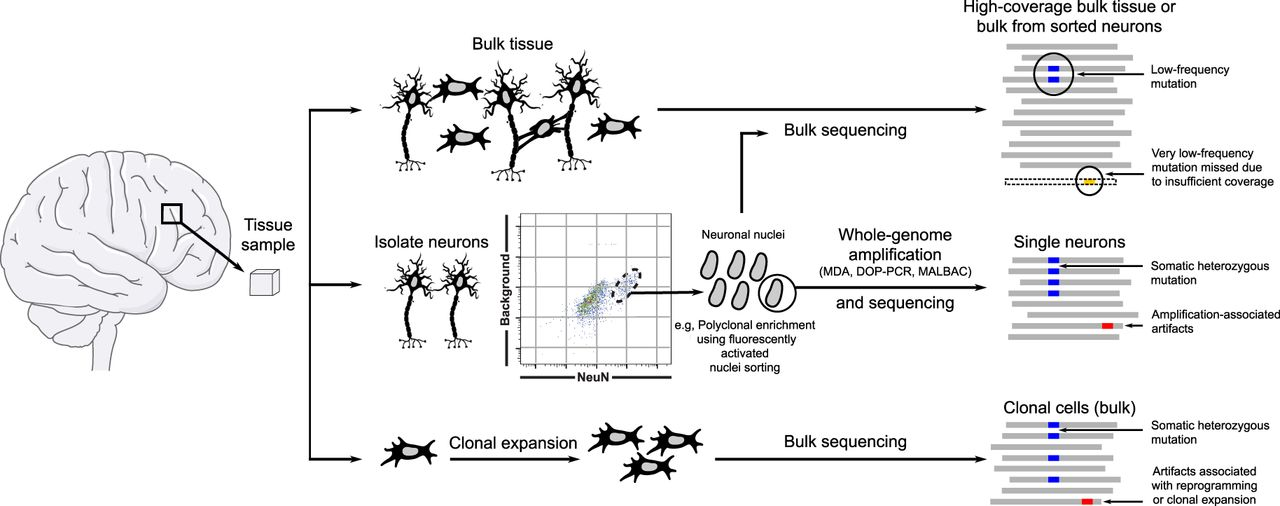
\includegraphics[width=1.0\textwidth]{figures/from-others/bsm-science-fig2.jpg}
\vfill
\tiny{McConnell et al Science 2017}
\end{frame}

%Slide: Proposed functional characterization
%The most interesting somatic variants will be characterized functionally in rhodents.
\begin{frame}{Proposed functional characterization}
\includegraphics[width=1.0\textwidth]{figures/from-others/bsm-science-fig4.jpg}
\vfill
\tiny{McConnell et al Science 2017}
\end{frame}

%Slide: Patterns of somatic mosaicism
%Work before the BSMN consortium already described some somatic variants in a
%normal individual by sequencing or genotyping single cells shown as dots.
%Some somatic variants like C1 and C2 were found in all those cells suggesting
%they are spread throughout the entire brain (but were absent from other body
%parts).  Other somatic variants like C6, C7, C8 and C10 were confined to 
%smaller regions.
\begin{frame}{Patterns of somatic mosaicism}
\includegraphics[height=0.7\textheight]{figures/from-others/lodato2015science-fig3b.png}
\vfill
\tiny{Lodato et al Science 2015}
\end{frame}

%Slide: Embryonic development
%To interpret the various patterns of somatic mosaicism we must consider
%embryonic development.  When a mutation occurs early, say, in the ectoderm
%around gastrulation then later on the somatic variant has a chance to spread out to
%much of the brain (which emerges from the neuroectoderm) but not to muscle
%and other mesodermal organs.
\begin{frame}{Embryonic development}
%gastrulation video
%https://www.youtube.com/watch?v=3AOoikTEfeo
%neurulation video
%https://www.youtube.com/watch?v=lGLexQR9xGs
\includegraphics[height=0.8\textheight]{figures/from-others/HumanEmbryogenesis.png}
\end{frame}

%Slide: Neocortical development
%But when a mutation occurs much later for instance in radial glia or an
%intermediate progenitor cell, then the somatic variant will be confined to
%the relatively few daughter cells, which are mostly neurons
%and marked by the expression of NeuN.
\begin{frame}{Neocortical development}
\includegraphics[height=0.8\textheight]{figures/from-others/doi_10_1016-j_cell_2011_06_030-fig4b-neocortical-development.jpg}
\vfill
\tiny{review: Cell.~2011;146(2):332}
\end{frame}

%Slide: Mutation rate
%Another question is the expected number of somatic mutations neurons. This
%meta analysis suggests that the mutation rate in the brain is low, comparable to
%that in the germline.  But while germline variants are hereditary, somatic
%variants aren't.  Therefore germline variants accumulate throughout
%generations and are expected to outnumber somatic variants in one neuron or a
%given set of neurons.
\begin{frame}{Mutation rate}
\includegraphics[width=0.8\columnwidth]{figures/from-others/lynch-evolution-of-mutation-rate-fig3.jpg}
\vfill
\tiny{Lynch Trends Genet.~2010}
\end{frame}

%Slide: Sequencing approaches to detect somatic variants
%Therefore one of the challenges in discovering somatic variants is to
%distinguish them from the much more common germline variants.  For example,
%our group uses bulk sequencing of neuronal nuclei that have been sorted out
%using NeuN, the marker mentioned before. For simplicity suppose that a
%variant is heterozygous. If the variant is germline then then the variant's
%allele frequency is 1/2 in our sample so we expect to see the variant in
%exactly half of the sequencing reads that map to its position in the
%reference genome.  But if the variant is somatic then its allele frequency in
%the sample is typically less then half so that we expect to see it in less than
%half of the reads, too.
%But due to sampling error at limited read depth we may easily mistake a high frequency somatic
%variant with a germline variant and we may easily miss a low frequency
%somatic variant.  Low read depth also makes sequencing errors appear as a low
%frequency somatic variants.  Therefore it is beneficial to
%sequence as deeply as our budget allows.
\againframe{bsm-methods}

%Slide: Mapped reads from a control individual
%We sequenced the whole genome of our NeuN plus samples at nearly 200x overall coverage.
%In blue you see how the read depth varies across the sex chromosomes in a
%control (not schizophrenic) individual.  The depth tends to be low on the Y
%chromosome confirming that the individual is female but the depth is not
%zero indicating mapping errors.  To help distinguish high frequency somatic
%variants from heterozygous germline variants we also sequenced a muscle
%sample and a sample of NeuN- brain cells from the same
%individual.
%The bar chart presents read counts of the reference allele C and the
%alternative allele (T) at this position (which is near the start of the X; show
%location on the left).  There are two pieces of evidence for this being a
%true somatic variant: first the allele is present on less than half of reads in
%the NeuN+ sample and second it is completely absent from the muscle sample.  Moreover, the
%fact that it's also present in the NeuN- brain sample suggests that the mutation
%occurred relatively early in development, perhaps during neurulation.
\begin{frame}[label=data-quantity]{Mapped reads from a control individual}
\begin{columns}[t]
\begin{column}{0.5\textwidth}
\includegraphics[width=1.0\columnwidth]{figures/2019-02-08-MSSM_106-depth/depth-plot-X-1.png}
\end{column}

\begin{column}{0.5\textwidth}
\includegraphics<2>[width=1.0\columnwidth]{figures/2019-02-08-somatic-calls-pileup/allele-counts-X-1355567-CT-1.pdf}
\end{column}
\end{columns}
\end{frame}

%Slide: Ongoing analyses
%Besides that control individual (MSSM_106) our group in the consortium analyzed samples from several
%control and SCZ brains from Sinai and U Pitt.
%Of course we did not attempt to find somatic variants by manual inspection
%of our mapped reads.  The genome is too large and the expected number of
%somatic variants is too little for that.  After mapping our reads we let
%several variant callers do this job.  Variant callers are statistical
%software tools that not only search for reads with some Alt allele (relative
%to the reference genome) and not only look at Ref and Alt read counts but
%also take additional evidence into account for or against a somatic variant: such as base
%quality and mapping quality.  Additionally, most of our callers can jointly
%analyze a NeuN+ sample together with either a muscle or NeuN- sample (but not
%both).  So what are the called variants and why were we not content with just one caller?
\begin{frame}{Ongoing analyses}
\includegraphics[width=1.0\columnwidth]{figures/2018-09-12-sequenced-individuals/summary-cmc-1.pdf}
\end{frame}

%Slide: Discordance between variant callers
%This is because callers are largely discordant.  Some of them called
%10 thousand(!) times more variants than others.  You might say that's OK if
%callers differ only in their specificity and sensitivity.  In that case their
%call sets should be nested in each other.  But this is not what we found
%suggesting that callers also differ in their biases: one tends to make one kind of mistake
%while another another kind of mistake.  In other words callers are
%largely complimentary to each other and would benefit from some kind of
%combination.
\begin{frame}<1-2>[label=discordance]{Discordance between variant callers}

\begin{columns}[t]
\begin{column}{0.5\textwidth}

\includegraphics<1-2>[width=1.0\columnwidth]{figures/2018-10-26-MSSM106-control-indiv/call-set-size-snvs-1.pdf}
\includegraphics<3>[width=1.0\columnwidth]{figures/2018-10-26-MSSM106-control-indiv/call-set-size-snvs-2.pdf}
\end{column}

\begin{column}{0.6\textwidth}

\includegraphics<2>[width=1.0\columnwidth]{figures/2018-10-26-MSSM106-control-indiv/venn-snvs-1.pdf}
\includegraphics<3>[width=1.0\columnwidth]{figures/2018-10-26-MSSM106-control-indiv/venn-snvs-PASS-1.pdf}
\end{column}
\end{columns}
\end{frame}

%Slide: Combination of call sets
%A popular way of combining callers is to take the intersection of call sets
%but that is not optimal in general.  Taking the union can be optimal if the
%callers have the same precision.  Precision is the fraction calls that are
%true.  Recall (or sensitivity) is the fraction of variants that are called.
%It follows from their definition that precision and recall can be evaluated
%only when the real variants are known in the data set.  Obviously this does
%not hold in the present case but later I will talk about a data set with
%known variants.
%So when precision and recall are unknown we may assume that callers differ in
%precision.  Then taking the union then amounts to inflating the higher
%precision callset with many false calls from the lower precision callset.
\begin{frame}{Combination of call sets}
\begin{columns}[t]
\begin{column}{0.5\textwidth}

\includegraphics<1-2>[height=0.6\textheight]{figures/Tnseq-4-strelka2Somatic-4-venn.png}
\end{column}

\begin{column}{0.4\textwidth}
\begin{center}
\only<1>{optimal, unrealistic}
\only<2>{not optimal, realistic}
\end{center}
\includegraphics<1>[width=1\columnwidth]{figures/by-me/precision-recall/pr-same-prec-2.pdf}
\includegraphics<2>[width=1\columnwidth]{figures/by-me/precision-recall/pr-realistic-2.pdf}
\end{column}
\end{columns}
\end{frame}

%Slide: Filtering of call sets
%Researchers often filter their callsets based on quality annotations attached
%to the callsets.  Filtering is perfect when we manage to remove all false
%calls while keeping all the true calls, so that the unknown precision is
%increased while the also unknown recall is fixed.  But in reality we can only
%increase precision at the expense of recall because our filters are
%heuristic.  That means we have only vague ideas on how quality annotations
%may help distinguish between true and false calls.  Nonetheless some callers
%offer a default filtering option and mark calls that PASS the filter.
\begin{frame}
\begin{columns}[t]
\begin{column}{0.4\textwidth}
perfect filtering

\includegraphics<1->[width=1\columnwidth]{figures/by-me/precision-recall/pr-realistic-2-filter-perfect.pdf}
\end{column}

\begin{column}{0.4\textwidth}
\only<2>{imperfect, heuristic filtering}

\includegraphics<2>[width=1\columnwidth]{figures/by-me/precision-recall/pr-realistic-2-filter-heuristic.pdf}
\end{column}
\end{columns}
\tiny
\setlength{\tabcolsep}{3pt}
\begin{tabular}{l|llllllll|}
\footnotesize &
\multicolumn{8}{c}{\footnotesize \texttt{TNseq.Mutect2.vcf}} \\
\hline
 & \#CHROM & POS & ID & REF & ALT & QUAL & FILTER & INFO \\
\textcolor{cyan}{\(c\)} &
\textcolor{cyan}{1} &
\textcolor{cyan}{50003788} &
\textcolor{cyan}{0} &
\textcolor{cyan}{A} &
\textcolor{cyan}{G} &
\textcolor{cyan}{0} &
\textcolor{cyan}{t\_lod\_fstar} &
\textcolor{cyan}{...;NLOD=30.4;TLOD=4.62} \\
\textcolor{cyan!50!brown}{\(d\)} &
\textcolor{cyan!50!brown}{1} &
\textcolor{cyan!50!brown}{50005034} &
\textcolor{cyan!50!brown}{0} &
\textcolor{cyan!50!brown}{G} &
\textcolor{cyan!50!brown}{T} &
\textcolor{cyan!50!brown}{0} &
\textcolor{cyan!50!brown}{t\_lod\_fstar} &
\textcolor{cyan!50!brown}{...;NLOD=33.27;TLOD=4.51} \\
\textcolor{cyan!50!brown}{\(e\)} &
\textcolor{cyan!50!brown}{1} &
\textcolor{cyan!50!brown}{50007349} &
\textcolor{cyan!50!brown}{0} &
\textcolor{cyan!50!brown}{C} &
\textcolor{cyan!50!brown}{T} &
\textcolor{cyan!50!brown}{0} &
\textcolor{cyan!50!brown}{PASS} &
\textcolor{cyan!50!brown}{...;NLOD=23.43;TLOD=10.97} \\
\textcolor{cyan!50!brown}{\(f\)} &
\textcolor{cyan}{1} &
\textcolor{cyan}{50008565} &
\textcolor{cyan}{0} &
\textcolor{cyan}{C} &
\textcolor{cyan}{A} &
\textcolor{cyan}{0} &
\textcolor{cyan}{PASS} &
\textcolor{cyan}{...;NLOD=7.69;TLOD=8.26} \\
\hline
% \vdots & \vdots & \vdots & \vdots & \vdots & \vdots & \vdots & \vdots & \vdots & \vdots & \vdots \\
\end{tabular}
\tiny
\\[1em]
\begin{tabular}{l|llllllll|}
\footnotesize &
\multicolumn{8}{c}{\footnotesize \texttt{strelka2Somatic.vcf}} \\
\hline
 & \#CHROM & POS & ID & REF & ALT & QUAL & FILTER & INFO \\
\textcolor{brown}{\(a\)} &
\textcolor{brown}{1} &
\textcolor{brown}{50003323} &
\textcolor{brown}{0} &
\textcolor{brown}{A} &
\textcolor{brown}{G} &
\textcolor{brown}{0} &
\textcolor{brown}{LowEVS} &
\textcolor{brown}{...;DP=274;MQ=59.86;...;SomaticEVS=0} \\
\textcolor{brown}{\(b\)} &
\textcolor{brown}{1} &
\textcolor{brown}{50003455} &
\textcolor{brown}{0} &
\textcolor{brown}{C} &
\textcolor{brown}{T} &
\textcolor{brown}{0} &
\textcolor{brown}{LowEVS} &
\textcolor{brown}{...;DP=226;MQ=59.9;...;SomaticEVS=0.65} \\
\textcolor{brown}{\(d\)} &
\textcolor{cyan!50!brown}{1} &
\textcolor{cyan!50!brown}{50005034} &
\textcolor{cyan!50!brown}{0} &
\textcolor{cyan!50!brown}{G} &
\textcolor{cyan!50!brown}{T} &
\textcolor{cyan!50!brown}{0} &
\textcolor{cyan!50!brown}{PASS} &
\textcolor{cyan!50!brown}{...;DP=278;MQ=59.95;...;SomaticEVS=9.04} \\
\textcolor{brown}{\(e\)} &
\textcolor{cyan!50!brown}{1} &
\textcolor{cyan!50!brown}{50007349} &
\textcolor{cyan!50!brown}{0} &
\textcolor{cyan!50!brown}{C} &
\textcolor{cyan!50!brown}{T} &
\textcolor{cyan!50!brown}{0} &
\textcolor{cyan!50!brown}{LowEVS} &
\textcolor{cyan!50!brown}{...;DP=192;MQ=59.88;...;SomaticEVS=4.19} \\
\hline
% \vdots & \vdots & \vdots & \vdots & \vdots & \vdots & \vdots & \vdots & \vdots & \vdots & \vdots \\
\end{tabular}
% ##INFO=<ID=SomaticEVS,Number=1,Type=Float,Description="Somatic Empirical
% Variant Score (EVS) expressing the phred-scaled probability of thecall being
% a false positive observation.">
\normalsize

\end{frame}

%Slide: Discordance between variant callers
%When we used the default filters the callers remained largely different both
%in the size and concordance of the call sets.  This suggests that the
%heuristic default filters are rather imperfect.
\againframe<3>{discordance}

%Slide: Discordance in Common Experiment
%An equally disappointing result came from the so called common experiment within
%the consortium.  In this experiment each of 5 groups sequenced the same
%sample and produced a call set by their preferred callers, heuristic filtering
%and combination.  The Venn diagram shows massive discordance among the
%groups' results suggesting many false calls.
\begin{frame}{Discordance in Common Experiment}
\includegraphics[height=0.65\columnwidth]{figures/from-others/bsmn-cs-callset-concordance.png}
\tiny{BSMN, unpublished}
\end{frame}

%Slide: Optimization of variant calling
%This lead the consortium to standardize and optimize somatic variant
%calling.  This methodological study is on its way and is planned to be published.
%The main approach of the consortium is to use the common sample and refine heuristic filtering
%by the validation of a limited number of calls.
%A complementary approach is taken by our group.  We use instead of a brain
%sample with real but unknown somatic variants an artificial sample with
%modeled and therefore known somatic variants.  This lets us quantify calling
%accuracy, which is essential for optimization.  Besides this we use a
%published machine learning technique that probabilistically and
%semi-automatically filters and combines call sets.
\begin{frame}{Optimization of variant calling}
\small
\begin{tabular}{r|cc}
& consortium & our group \\
\hline
somatic variants in sample & real, unknown & modeled, known \\
validation & targeted resequencing & not needed \\
reported accuracy & qualitative & quantitative \\
variable selection (filtering) & heuristic & probabilistic, manual \\
filter setting & heuristic & probabilistic, automated \\
\end{tabular}
\end{frame}

%Slide: Modeling somatic variants
%We mixed DNA of four individuals (grandprents of the much studied CEPH/Utah
%pedigree) in different proportions to model somatic variants at various
%allele frequencies.  A modeled somatic variant is a germline variant present in
%one or more of the the individuals (but not in all of them).  Its allele
%frequency is determined by the mixing proportions, which individuals it is
%present in and with what zygosity.  The advantage of such modeled somatic
%variants is that they are known with high accuracy because the underlying
%germline variants have been called before mixing the samples.
\begin{frame}[label=benchmark]{Modeling somatic variants}
\begin{center}
\begin{columns}[t]
\begin{column}{0.5\textwidth}

\includegraphics[width=1\textwidth]{figures/from-others/ceph-utah-pedigree-1463.png}
\end{column}

\begin{column}{0.5\textwidth}

\small
{\onslide<1->
\begin{tabular}{cccc}
genome & mix1 & mix2 & mix3\\
\hline
NA12889 & 4 & 2 & 0\\
NA12891 & 8 & 4 & 0\\
NA12890 & 16 & 8 & 0\\
NA12892 & 72 & 86 & 100\\
\hline
total & 100 & 100 & 100\\
\end{tabular}
}
\end{column}
\end{columns}
\end{center}
\end{frame}

%Slide: Callers in precision-recall space
%Since the somatic variants are known we can evaluate the performance in terms
%of precision and recall of our
%somatic variant callers on the DNA mixes.  The
%callers were used with their default filters.
%We can draw the following conclusions from this plot.
%The performance of all callers
%First, if we forget lofreqSomatic for a second then strelka2Somatic performs best,
%then TNseq.Mutect2, then somaticSniper and finally strelka2Germline.
%Second, we can't say that lofreqSomatic performs better or worse than any other
%caller because it is the most precise but least sensitive caller.
%Third, the callers differ greatly in precision.  Therefore their combination
%by union would be far from optimal.
\begin{frame}[label=precrecall]{Callers' performance with default filters}
\includegraphics[width=1\textwidth]{figures/from-others/chaggai-precision-recall.png}

\tiny{Chaggai Rosenbluh}
\end{frame}

%Slide: Filtering and combination of callers
%Here I show two approaches to combining callers.  The problem with the
%traditional is that it's not clear how to adjust filters in real world
%datasets when precision is unknown.  Luckily the probabilistic approach,
%implemented by VariantMetaCaller was designed to estimate precision for each
%call after ranking calls according to their probability of being true.
%Moreover VariantMetaCaller also combines callers when it estimates
%probabilities using machine learning.
\begin{frame}{Filtering and combination of callers}
\begin{columns}[b]
\begin{column}{0.5\textwidth}
\begin{center}
{\large traditional}

{\footnotesize
\begin{enumerate}
\item select precision \emph{a priori}
\item adjust filters---\alert{but how?}
\item combine callers
\end{enumerate}
}
\end{center}
\includegraphics[width=0.9\columnwidth]{figures/by-me/precision-recall/pr-same-prec-unfiltered.pdf}
\end{column}

\begin{column}{0.5\textwidth}
\begin{center}
{\large probabilistic}

{\footnotesize
\begin{enumerate}
\item combine callers for each call
\item sort calls by their probability
\item filter at any precision
\end{enumerate}
}
\end{center}
\includegraphics[width=0.9\columnwidth]{figures/by-me/precision-recall/pr-pass-vmc.pdf}
\end{column}
\end{columns}
\end{frame}

%Slide: Filtering and combination of callers
%The black line shows the precision-recall curve for the combined caller
%created by VariantMetaCaller.  The software is not fully configured yet which
%explains why currently it is outperformed by strelka2Somatic and
%TNseq.Mutect2 at the precision of those two callers.  Configuration is in
%progress.  But we can already use its feature of precision based filtering.
%For instance if we want an intermediate precision between lofreqSomatic and
%strelka2Somatic (or equivalently TNseq.Mutect2) then VariantMetaCaller can
%give us the corresponding callset.
\againframe{precrecall}

\begin{frame}{Impact of alternative allele frequency}
\includegraphics[width=0.9\textwidth]{figures/from-others/chaggai-recall-aaf.png}

\tiny{Chaggai Rosenbluh}
\end{frame}

\begin{frame}{Summary}
\begin{enumerate}
\item \alert{somatic mutations} in neurological psychiatric disorders\\
\emph{Brain Somatic Mosaicism Network}
\item somatic mutations in \alert{schizoprhenic} and control brains\\
\emph{our group}
\item workflows for somatic variant calling: \alert{discordance}
\item workflow characterization and \alert{optimization}
\begin{itemize}
\item heuristics---\emph{BSMN}
\end{itemize}
\item probabilistic approach---\emph{our group}
\begin{itemize}
\item benchmark data \(\Rightarrow\) precision--recall
\item \alert{machine learning}
\item input: base/mapping/calling \alert{quality annotations}
\end{itemize}
\end{enumerate}
\end{frame}

\begin{frame}{BSMN consortium team}
Brain Somatic Mosaicism Network
\footnotesize
\begin{tabular}{rl}
\hline
P.I. & institution \\
\hline
\alert{Chess} & \alert{Icahn School of Medicine at Mount Sinai}\\
Gage & Salk Institute for Biological Studies\\
Gleeson & University of California, San Diego\\
Moran & University of Michigan\\
\alert{Park} & \alert{Harvard University}\\
Pevsner & Kennedy Krieger Institute\\
Sestan & Yale University\\
Vaccarino & Yale University\\
\alert{Walsh} & \alert{Boston Children's Hospital}\\
Weinberger & Lieber Institute for Brain Development\\
\end{tabular}
\vfill
\begin{columns}[t]
\begin{column}{0.3\textwidth}
\begin{center}

\includegraphics[width=0.5\columnwidth]{figures/from-others/NIH_logo.png}
\end{center}
\end{column}

\begin{column}{0.3\textwidth}
\begin{center}

\includegraphics[width=0.5\columnwidth]{figures/from-others/nda.pdf}

NIMH Data Archive
\end{center}
\end{column}

\begin{column}{0.3\textwidth}
\begin{center}

\includegraphics[width=0.5\columnwidth]{figures/from-others/synapse.pdf}

Synapse
\end{center}
\end{column}
\end{columns}
\end{frame}
\end{document}


\begin{columns}[t]
\begin{column}{0.5\textwidth}

\end{column}

\begin{column}{0.5\textwidth}

\end{column}
\end{columns}
